\cotefile{67}
\scanpage{19}
\mspage{\handwritten{4}}

uncer $\underline{\mathrm R}^{+\deleted{\unsure{\times|*}}}$, which plays here the role of the parameter space of \inserted{all} possible (non degenerate) ``radii'' at $s_i$. If we admit also radius zero, we accordingly get a parameter space $R_i^{\wedge}$, which may be viewed as a torsor of sorts \deleted{over}\handwritten{under} $\underline{\mathrm R}^{+}$. Thus the set of radii for a given admissible system of discs $D_i$ around the points $s_i$ may be viewed as a point of the product-space
\[
r=(r_i)_{i\handwritten{\in} I}\handwritten{\in} R^{\wedge}=\mathop{\handwritten{\prod}}\limits_{i\handwritten{\in} I} R_i^{\wedge}.
\]
My expectation is that an admissible set of discs $(D_i)$ is well determined by the knowledge of the corresponding set \inserted{\handwritten{$r$}} of radii \deleted{$\unsure{r}$}, and moreover that a given set \inserted{\handwritten{$r$}} of radii \deleted{$\unsure{r}$} corresponds to \deleted{a}\inserted{an admissible} system of \deleted{admissible} discs iff it satisfies a set of unequalities
\[
r_i\handwritten{<\rho}_i,
\]
where
\[
\handwritten{\rho}=(\handwritten{\rho}_i)_{i\handwritten{\in} I}\handwritten{\in} R=\mathop{\handwritten{\prod}}\limits_{i\handwritten{\in} I} R_i
\]
is \deleted{a}\inserted{\handwritten{some}} fixed system of radii, corresponding to a fixed system of choices of hermitian metrics in the tangent spaces $T_{s_i}$.

I now see that this ``expectation'' does'nt quite match \inserted{with} the previous one, about a ``natural operation'' of $(\underline{\mathrm P}^{\unsure{+|*}})^I$ upon $\overset{\handwritten{\sim}}{\mathrm{MB}}$, having certain properties - it would match only if all \handwritten{$\rho_i$} where equal to $+\infty$ (hence not in $R_i$ itself strictly speaking). I must confess I did'nt look too thoroughly yet at the situation, and moreover I've been busy with rather different kind of things for the last two or three months, and lost \inserted{\handwritten{contact}} a little\handwritten{...} \deleted{contact.} What is clear however is that the main key to an understanding of the general situation, is in an understanding of the basic particular case of Thurston's pants. If we number $0,1,\infty$ the three ``holes'' of such a pant, the surface $X^{\wedge}$ can be identified canonically to the Riemann sphere, and the basic question then is to understand how the pant is imbe\handwritten{d}ded in this sphere \handwritten{$\Sigma$}, as a complement of \deleted{(open)} the union of (open) discs around the points $0,1,\infty$, these discs forming an ``admissible system''. So the main question is about understanding the structure of all possible admissible systems of three discs on \handwritten{$\Sigma$}.

P\deleted{\unsure{y}}uzzling a little about this problem, the following model came to my mind (corresponding to \handwritten{``}limiting radii\handwritten{''} $\handwritten{\rho}_i$ which are \uline{finite}, not infinite). I view \handwritten{$\Sigma$} as endowed with it's usual euclidean metric, for which the real projective line is a great circle, with $0,1,\infty$ at equal distance from each other on this equator. These points may be viewed as the centers of three ``orange \deleted{quarters}\inserted{\handwritten{slices}}'', making up a cellular subdivision of \handwritten{$\Sigma$}, where the common boundary of two among the ``\deleted{quarters}\inserted{\handwritten{slices}}'' $Q_i$ $(i\handwritten{\in\{}\unsure{C|0},1,\infty\handwritten{\}})$ is a half-great circle passing in between $s_i$ and $s_j$ at equal
% archive sheet number: 18

\scanpage{20}
\mspage{\handwritten{5}}

distance from both, these three half-circles joining at the two poles $P^+$ and $P^-$. The ``disc'' $Q_i$ around $s_i$ has a conical structure around $s_i$ (as has any conformal pointed disc), and we may take the concentric \deleted{\unsure{disc|dis-|discs}} discs $\handwritten{\lambda}_i Q_i$ with
\[
0\mathrel{\overset{\deleted{\unsure{i}}}{\handwritten{<}}}\handwritten{\lambda}_i\handwritten{<}1.
\]
T\deleted{\unsure{t}}he model I had in mind was that the (non degenerate) admissible systems of discs around the points $s_i$ $(i\handwritten{\in\{}0,1,\infty\handwritten{\}})$ \deleted{\unsure{wh}}are exactly the systems of discs $\handwritten{\lambda}_i Q_i$, with $\handwritten{\lambda}_i$ as above. (If we allow some discs to be degenerate, this means that instead of the unequality above we merely demand $0\handwritten{\leq\lambda}_i\handwritten{<}1$, $0$ not excluded.)

This model, if correct, would give a rather precise description of the inclusion relationships between pants, when these are considered as embedded in the sp\deleted{\unsure{b}}here. The intersection of all would be this system of th\deleted{\unsure{ese}}ree half circles $C_i$, and the two poles $P^+,P^-$ would play a significant role in the geome\handwritten{t}ry of the pants, from this point of view. But it does'nt seem that neither those half circles (which need not be geodesical I guess)\handwritten{,} no\deleted{t}r the two poles\handwritten{,} have ever been described as intrinsically associated to a pant. Of course, this model would give alternative ``parameters'' $\handwritten{\lambda}_i$ for describing a pant, which are best suited for grasping the pants in terms of spherical geometry. The next question would be an understanding of the relationship between these parameters, and Thurston's $\handwritten{\ell}_i$. Maybe it is unreasonable to expect that for given index $i\handwritten{\in\{}0,1,\infty\handwritten{\}}$, the length $\deleted{\handwritten{\lambda}}\handwritten{\ell}_i$ depends only on $\handwritten{\lambda}_i$ and not on the other parameters $\handwritten{\lambda}_j$ - and for this reason, \deleted{\unsure{it is}} the in\handwritten{t}uition at the beginning of this letter, using Thurston's coordinate functions and notably the $\handwritten{\ell}_i$'s to get a fibration structure on $\widetilde{\mathrm{MB}}$ over $\widetilde{\mathrm M}$, in terms of a given decomposition of $X_{\unsure{o|0}}$ into pants, is probably not really relevant, namely it is non intrinsic. Assuming the model I am suggesting is correct, the accurate description \deleted{\unsure{but}} of $\widetilde{\mathrm{MB}}$ in terms of $\widetilde{\mathrm M}$ would be
\[
\widetilde{\mathrm{MB}}\handwritten{\simeq}\widetilde{\mathrm M}\mathbin{\mathrm{x}}\handwritten{[}0,1\handwritten{[}^{I},
\]
where the second factor on the right hand sight refers to the system of multipliers $\handwritten{\lambda}_i$ $(i\handwritten{\in} I)$, tied to the $r_i$ above by $r_i=\handwritten{\lambda}_i\handwritten{\rho}_i$.

My question of course is whether you have any information or idea to propose, especially on the basic problem of relying pants to spherical geometry, and more specifically, \deleted{\unsure{if}}\handwritten{wh}ether the model above is likely to hold, or is defintely false. Also, one difficulty we found with hyperbolic geometry of conformal surfaces, \inserted{\handwritten{is}} that apart from existence and unicity of the hyperbolic structure (compatible with the given conformal one and for which the boundary is geodesic), there seems to be little
% archive sheet number: 19

\scanpage{21}
\mspage{\handwritten{6}}

hold on more specific properties. As an example, starting with a \inserted{compact} conformal surface with boundary $X$ (a pant, say), of hyperbolic type, and removing an \deleted{-}(open) ``collar'' a\deleted{\unsure{p|r}}roun\deleted{\unsure{f|d}}d the bou\inserted{n}dary, we get another surface with boundary $X'$ - what about the relation \deleted{of}\inserted{between} the two corresponding metrics ? Assuming the model \deleted{\unsure{r}}for pants above is correct, it would be nice to have an explicit expression of the metric of a pant in terms of the parameters $\handwritten{\lambda}_i$,

With my thanks for your attention, and for whatever comment you\\
will care to make, very sincerely ypur's\\
% archive sheet number: 20

\scanpage{24}
Métriques canoniques sur surfaces conformes
% archive sheet number: 26

\scanpage{25}
a) deux \unsure{réellifications|réllifications|réalifications} de types opposés, compatibles i.e une paire compatible d'antipodisme et \unsure{inversion}

b) Métrique sphérique $+$ grd cercle

c) cercle $+$ structure torique compatible dessus i.e. \deleted{\unsure{anti}}involution \deleted{\unsure{de cercle}}\inserted{avec pts fixes}, et paire des points conjugués par la dite

d) Tore compact $T\subset G=\mathrm{Aut}^{+}(X)$, $+$ orbite de $X\setminus X^T$ sous $T$ (i.e. orbite non réduite \unsure{à|;} un point)

d$'$) paire des pts. $\{z,z'\}\subset X$, $+$ orbite de $X\setminus\{z,z'\}$ du tore compact unique $T\subset G$ qui fixe $z,z'$.
% archive sheet number: 27

\scanpage{26}
\[
u_+ \qquad \frac{1}{2}(u_++u_-)
\]

\[
\underset{m}{\underset{\rule{.35pt}{2pt}\rule{4.4em}{.35pt}\rule{.35pt}{2pt}}{(x+\tfrac{1}{2}y)}}u_+
+\underset{n}{\underset{\rule{.35pt}{2pt}\rule{2em}{.35pt}\rule{.35pt}{2pt}}{\tfrac{1}{2}y}}u_-
\]

\figure{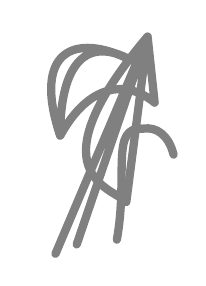
\begin{tikzpicture}[x=.6cm,y=.6cm,line cap=round,line join=round]
\draw[gray,line width=3pt] (.1,2.5) .. controls (-.5,4.3) and (.4,4.7) .. (1.6,4.1) .. controls (.7,4.6) and (.1,4.1) .. (.1,2.5) .. controls (.7,3.6) and (1.5,3.7) .. (2.1,3.2) -- (1.95,4.6) -- (.45,.2) -- (1.95,4.6) -- (1.5,1.1) .. controls (1.2,1.4) and (-.5,1.7) .. (1.95,4.6) -- (0,0);
\draw[gray,line width=3pt] (1.3,.3) .. controls (1.55,1.7) and (1.15,2.7) .. (1.85,2.65) .. controls (2.15,2.7) and (2.4,2.5) .. (2.5,2.1);
\end{tikzpicture}}

\diagram{\begin{tikzcd}[ampersand replacement=\&,column sep=small]
0 \arrow[r] \& \Pi \arrow[r] \& V \arrow[r,dash] \& E \arrow[r] \& 0
\end{tikzcd}}

\[
H^1(\deleted{\unsure{\langle}}\gamma,E)\xrightarrow{\sim} H^{\unsure{2}}(\gamma,\Pi)\simeq \Pi^{\gamma}/(1+\sigma)(\Pi)
\]

\[
z\longmapsto\exp 2i\pi z
\]

\figure{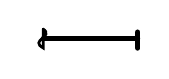
\begin{tikzpicture}[x=1cm,y=1cm,line cap=round]
\draw[line width=1.8pt] (0,0)--(1.2,0);
\draw[line width=1pt] (0,.12)--(0,-.12) .. controls (-.18,-.02) and (.14,.02) .. (0,.12);
\draw[line width=2pt] (1.2,-.12)--(1.2,.08);
\end{tikzpicture}}
% archive sheet number: 28

\scanpage{27}
\mspage{\textcircled{1}}

$X$ surface \deleted{conforme}\inserted{hol $0$-connexe} (pas néc cpte)
\margin{\uline{NB} Ici ``surface'' sous-entend ``séparée''}

$\widetilde X$ rev. universel

\uline{Th} Conditions équivalentes

(i) $X$ n'est pas isom à une des trois surfaces $\mathbb P^1_{\mathbb C}$, $\mathbb E^1_{\mathbb C}=\mathbb P^1_{\mathbb C}\setminus\{\infty\}$, $\mathbb G_{m\,\mathbb C}=\mathbb P^1_{\mathbb C}\setminus\{\infty,0\}$, ni à une courbe elliptique complexe

(ii) $\widetilde X$ est isomorphe à $H$ (demi-plan de Poincaré)

(iii) Toute application holomorphe $\mathbb C\longrightarrow X$ est constante

(iv) [Si $X$ est un ouvert \deleted{de}d'une droite projective complexe $\unsure{L|]}$ (resp. d'une droite affine complexe $L$)]
\[
\mathrm{Card}\,(\deleted{\unsure{L|X}}X'\setminus\deleted{L}X)\geq 3\quad(\text{resp. }\mathrm{Card}(\deleted{\unsure{L|X}}X'\setminus X)\geq 2).
\]

\deleted{(iv$'$) [Si $X$ est un ouvert de la surface holomorphe \unsure{compacte|connexe|conforme} $X'$}

(v) [Si $X=\widehat X\setminus S$, $\widehat X$ compacte \inserted{genre $g$}, $S$ finie \inserted{card $\nu$}] $\deleted{3}2g+\nu\geq 3$ \inserted{i.e. $(g,\nu)\notin\{(0,0),(0,1),(0,2),(1,0)\}$ i.e. $\unsure{\chi_{!}|\chi}(X)<0$}

\uline{Déf} On dit alors que $X$ est ``hyperbolique''

\uline{Corollaire 1} Un ouvert $0$-connexe d'une surface hol. hyperbolique est hyperbolique

\uline{Corollaire 2} Soit $X$ surface hol. \uline{\deleted{\unsure{con}}à bord}, \deleted{$\unsure{0{-}\mathrm{co}}$} connexe, avec $\partial X\neq\varnothing$. Alors $\mathrm{Int}\,X$ est hyperbolique
% archive sheet number: 29

\scanpage{28}
\mspage{\textcircled{2}}

les surfaces suivantes :

a) le plan projectif réel ($\simeq$ Sphère conforme/antipod) et le plan projectif réel privé d'un point (dont les rev. universels sont resp. $\simeq\mathbb P^1_{\mathbb C}$ et $\simeq\mathbb G_{m\,\mathbb C}$).

b) Les surfaces conformes associées aux courbes \deleted{elliptiques}\inserted{lisses géom. \unsure{intègres|connexes}} réelles $E$ \inserted{de genre $1$} telles que $E(\mathbb R)=\varnothing$, en posant \deleted{$\unsure{E\subset E|E\subset\mathbb C|E\in\mathbb C|E(\mathbb C)}$}
\[
X=E(\mathbb C)/\text{conj. complexe}.
\]

On trouve que les $E$ en question, à \unsure{trans|torsion|isom} près, sont les $E_a^{!}$, $a\in\mathbb R^{*+}$ ..

\noindent\rule{\linewidth}{.35pt}

\uline{Question des\inserted{la} métriques riemanniennes canoniques sur une surface conforme}

(sans bord pour commencer)

\textcircled{1} Cas hyperbolique, Il y a une métrique canonique, à courbure constante de valeur $-1$, déduite par descente du revêtement universel $\widetilde X$.

\uline{Métrique hyperbolique}
% archive sheet number: 30

\scanpage{29}
\mspage{3}

déterminée par la condition que l'aire totale de $X$ soit $=1$. On trouve une \uline{métrique plate} caractérisée par la condition d'être invariante par translation, et d'aire \deleted{\unsure{volume}} totale égale à $1$ -- donc stable par tt autom conforme (pas seulemt holomorphe). Il s'ensuit que dans le cas non orienté, la métrique canonique de $X^{\mathrm{or}}$ (qui est une courbe elliptique $/\mathbb C$) se descend à $X^{\unsure{\mathrm{or}|n}}$.

$\deleted{\unsure{3}}2'$) Cas $X\simeq\mathbb C^*$, ou \inserted{$X\simeq$} plan projectif réel privé d'un point [i.e $X$ non orientable et $X^{\mathrm{or}}\simeq\mathbb C^*$]. Comme dans 2, dans le cas $X\simeq\mathbb C^*$, \deleted{plus intrinsèquement $X\simeq$} \deleted{\unsure{de|par}}par descente à partir du rev. universel on trouve une métrique canonique mod multiplication par un scalaire $>0$, \uline{métrique plate} également. \deleted{\unsure{Comme}} les autom de $\mathbb C^*$ \inserted{sont} \deleted{\unsure{provient|peuvent}}\inserted{\unsure{soit|être|hol}} de la forme $z\longrightarrow az$, soit $z\mathrel{\unsure{-|\to}}a/z$, qui conservent la métrique [car sur $\widetilde{\deleted{\mathbb C}X}\simeq\mathbb C$ cela correspond à des autom $z\mathrel{\unsure{-|\to}}z+\alpha$, $z\mathrel{\unsure{\vdash\!\dashv|\mapsto}}-z+\alpha$], Donc en divisant la métrique sur $\mathbb C^*$, \deleted{de façon}\inserted{\unsure{en|on}}
% archive sheet number: 31

\scanpage{30}
\mspage{4/}

\deleted{\unsure{par}}en la normalisant \inserted{p. ex.} de telle façon que la longueur du cercle $|z|=1$ soit $\deleted{2\pi}1$, \margin{C'est la métrique déduite de \unsure{l'unité que|la métrique|l'unitaire} hermitienne canonique $z\bar z$ sur $\mathbb C$, via $z\mapsto\exp 2i\pi z$, de $\mathbb C$ sur $\mathbb C^*$.} on la définit sur toutes les $X\simeq\mathbb C^*$ du $=$ fait. D'ailleurs l'\unsure{anti-automorphisme|antiautomorphisme} $z\mapsto\bar z$ \deleted{\unsure{respecte}} conserve la mesure, donc si $X\simeq\mathbb C^*$, \uline{tt} autom. conforme respecte \deleted{\unsure{la}}la mesure canonique.

Il en résulte que dans le cas non orienté $X\simeq$ plan projectif réel moins $1$ pt, on peut descendre à partir de $X^{\mathrm{or}}$ et on trouver encore une métrique canonique plate, stable par tous les automorphismes conformes.

$\deleted{\unsure{3}}2''$) Cas $X\simeq\mathbb E^1_{\mathbb C}$. \unsure{``}Les métriques riemanniennes sur une \deleted{\unsure{vect}} droite vectorielle \unsure{1|$L$} complexe \inserted{$L$}, associées aux structures hermitiennes \inserted{déf. pos} sur $L$, (\deleted{\unsure{elles|celles}} elles sont toutes proportionnelles) ne sont \uline{pas} invariantes par autom \deleted{\unsure{de}}\inserted{hol} $L$, mais seulemt par le sous-groupe engendré par les translations, et les \deleted{\unsure{multipl.|autres}} homothéties par des $u\in\mathbb U=\{z\in\mathbb C\mid |z|=1\}$; elles sont quasi-invariantes par autom quelconques (lesquels sont \uline{affines}). Donc sur une $X\simeq\mathbb E^1_{\mathbb C}$, on peut définir, non \uline{une} métrique
% archive sheet number: 32

\scanpage{31}
\mspage{5/}

canonique stable par translations etc, mais une classe de telles mod homothétie par $c\in\mathbb R^{*+}$ -- ces métriques sont caractérisées par la condition d'être invariantes par translation [\uline{NB} $X$ a automatiquement une structure de droite affine sur $\mathbb C$]. Ces métriques \deleted{sont \unsure{caractérisées}} ne dépendent que de la structure conforme sous-jacente.

3) \uline{Cas} \deleted{\unsure{de la sphère} $X\simeq\mathbb P^1_{\mathbb C}$} $X\simeq$ \deleted{\unsure{droite|sphère}}plan projecti\deleted{ve}f réel. Dans ce \deleted{premier} \deleted{\illegible{1}} cas, $X^{\mathrm{or}}$ est une droite projective complexe munie d'un antiautomorphisme invol. $\sigma$ \uline{sans pt fixe} (antipodisme), ou ce qui revient au $=$, d'une métrique ``euclidienne sphérique'' compatible avec sa structure conforme. [Celle-ci, \deleted{étant stable} \inserted{\unsure{supp.|sera} normalisée} \deleted{par l'antipodisme,} \inserted{par la condition} que l'aire de la surface soit $=1$] É\deleted{\unsure{tant}}tant invariante par l'antipodisme, cette métrique se descend à $X$.

$3')$ Cas $X\simeq\mathbb P^1_{\mathbb C}$. Il n'y a pas de métrique riemannienne sur $X$, invariante [ou quasi-invariante] par tt automorphisme -- \unsure{dem.|demande|donc} une structure suppl. sur $X$

% archive sheet number: 33

\scanpage{32}
\mspage{6)}

il n'est pas possible d'y introduire une métrique riemannienne canonique, même modulo $\mathrm c^{\mathrm{te}}$. Considérons cependant la donnée d'une structure supplémentaire du type
\[
H\subset\mathrm{Aut}_{\mathrm{conf}}(X)=G
\]
où $H$ est un sous-groupe \uline{compact} de $\mathrm{Aut}_{\unsure{G|0}\,\mathrm{conf}}(X)$. Condition \uline{nécessaire} pour que $H$, supposé fermé, invarie une métrique euclidienne sphérique comp. avec la str. conforme). Soit $H^+=H\cap\mathrm{Aut}^+(X)$ (ss-groupe des autom qui conservent l'orientation). OPS $X=\mathbb P(V)$, $V$ vectoriel complexe de rg $2$, \deleted{\unsure{alors|étant}} soit $\overset{\deleted{\unsure{\sim}}}{\widetilde H}$ l'image inverse de $H^+$ dans $\unsure{\mathrm{SL}_{\mathbb C}(2,V)|\mathrm{SL}(2,V)|\mathrm{SL}(V)}$, c'est donc un sous-groupe cpt, qui invarie nécessairement une forme hermitienne déf. pos. sur $V$, donc la métrique sphérique corr. sur $X$ \inserted{(normalisée par la condition $\int_X dx=1$)}. Dans le cas où \deleted{cette métrique} \inserted{la métrique} hermitienne invarie est unique mod $\mathrm c^{\mathrm{te}}$, on trouve donc une métrique \inserted{sphérique normalisée} canonique sur $X$, définie par la \inserted{seule} donnée de $H^+$. Cette métrique sera $=$ invariante par $\mathrm{Norm}_G(H^+)\deleted{\unsure{\subset\mathrm{Aut}}}$, et a fortiori par $H$, et est encore caractérisée par cette condition.

% archive sheet number: 34

\scanpage{33}
\mspage{7)}

Nous allons maintenant examiner de plus près le cas où \deleted{$H^+$ \unsure{invarie}} $\mathrm{Herm}^{++}(V)^{H^+}$ n'est pas réduit à une demi-droite. On vérifie aisément que cela revient à dire que $H^+$ \deleted{\unsure{est tel}} fixe deux pts distincts $z,z'$ de $X$, donc est contenu dans le sous groupe de $G^+$ \deleted{défini} formé des pts qui fixent $z,z^{\unsure{'|*}}$, lequel est isom à $\mathbb C^*$, \deleted{\unsure{et il a}} \inserted{et admet un} unique sous-groupe cpt maximal \deleted{$\unsure{Y}$ \unsure{isom. à}} \inserted{$T$ isom à $\mathbb U$}. \deleted{Dans ce cas Les métriques invariées par}

Si $H^+\ne\{1\}$, \inserted{[alors $\{z,z'\}$ donc $T$ est uniquement déterminé]} les métriques invariées par $H^+$ sont aussi celles invariées par $T\supset H^+$, \margin{\uline{à vérifier}} et elles sont en corr. $1$-$1$ avec les \deleted{trajectoires} \inserted{orbites} de $T$ dans $X^*=X\smallsetminus\{z,z'\}$, [NB $T$ opère librement sur $X^*\deleted{\unsure{\setminus\{z}}$].

La relation est obtenue en associant à tte métrique invariée par $T$, \deleted{l'équateur} le grand cercle ayant comme pôles $z,z'$, lequel est une \deleted{trajectoire} \inserted{orbite} sous $T$. En particulier, tte orbite \inserted{de $X^*$} sous $H^+$ (étant contenue dans une unique orbite de $T$) définit une telle métrique.

Si $H=H^+$, il n'y a \deleted{\unsure{pas}} rien à ajouter. Dans le

% archive sheet number: 35

\scanpage{34}
\mspage{8)}

cas contraire, distinguons deux cas.

a) $H^+=\{1\}$, donc $H=\{1,\sigma\}$, où $\sigma$ est une anti-involution.

1) Si \deleted{$\unsure{\sigma}$} $X^\sigma=\varnothing$, $\sigma$ fixe une métrique sphérique normalisée unique, OK.

2) Si $X^\sigma\ne\varnothing$ i.e. $\sigma$ une inversion, alors le choix d'une métrique sphérique comp. avec $\sigma$ revient à celui d'une paire de pts de $X$ conjugués sous $\sigma$. En particulier, le choix d'un point \inserted{$x$} de $X$ tel que $\sigma x\ne x$ définit une telle métrique sphérique.

b) $H^+\ne\{1\}$. Considérons le \inserted{unique} tore \deleted{\unsure{gr}} compact de dim $1$ $T$ qui contient $H^+$, et $T.H=N$, ext. de \deleted{$\unsure{\mathbb Z}$} $\mathbb Z/2\mathbb Z$ par $T$. Les elts \deleted{\unsure{de}} $\sigma$ de $N^-$ fixent $z,z'$, ou les intervertissent, suivant que l'élt $\ne1$ de $N/T$ opère trivialement sur $T$, ou par symétrie $t\mathrel{\unsure{\vdash\!\dashv|\mapsto}}t^{-1}$.
% slanted
\margin{\uline{C'est l'inverse !}}
Dans le premier cas l'ext. $N$ de \inserted{$\gamma=$}$\mathbb Z/2\mathbb Z$ par $T$ est triviale
\[
(H^2(\gamma,T)\simeq T^\sigma/N_\sigma(T)=T/T^2\simeq0)
\]
dans le deuxième cas on trouve
\[
H^2(\gamma,T)\simeq T^\sigma/N_\sigma(T)\simeq \underbrace{{}_2T}_{\mathbb Z/2\mathbb Z}/0\simeq\mathbb Z/2\mathbb Z,
\]

1) $N$ ext. \uline{centrale} de $\deleted{\unsure{\mathbb Z|\gamma}}\gamma$ par $T$, donc $N\simeq T\times\underset{\substack{\Vert\\\{1,\sigma\}}}{\gamma}$ ($\frac12$ direct) engendré par $T$ et un $\sigma$ \deleted{qui} anti-involutif qui \deleted{fixe $z,z'$} intervertit $z,z'$. \deleted{On voit que} \deleted{\unsure{géodésique}} celle-ci est une inversion, \deleted{\unsure{ayant|dont|qui}}

\figure{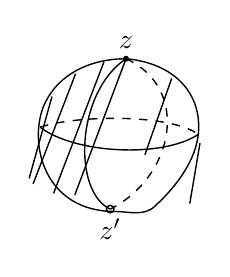
\begin{tikzpicture}[x=1cm,y=1cm,line width=.5pt]
\draw (0,.05) .. controls (-.88,.05) and (-1.1,.88) .. (-.91,1.38) .. controls (-.73,1.81) and (-.29,1.99) .. (.14,1.99) .. controls (.77,1.93) and (1.1,1.54) .. (1.06,1.05) .. controls (1.03,.70) and (.78,.37) .. (.52,.13) .. controls (.38,-.02) and (.18,.05) .. (0,.05);
\draw (.14,1.99) .. controls (-.50,1.56) and (-.54,.30) .. (-.06,.08);
\draw[dashed] (.14,1.99) .. controls (.97,1.61) and (.75,.49) .. (-.06,.08);
\draw (-.95,1.12) .. controls (-.52,.79) and (.59,.72) .. (1.06,1.03);
\draw[dashed] (-.95,1.12) .. controls (-.52,1.27) and (.68,1.30) .. (1.06,1.03);
\draw (-1.09,.47)--(-.80,1.51) (-1.04,.40)--(-.50,1.80) (-.78,.28)--(-.14,1.95) (-.51,.26)--(.14,1.99) (.38,.77)--(.72,1.74) (.95,.15)--(1.08,.92);
\fill (.14,1.99) circle (.038) node[above] {$z$}; \draw (-.06,.08) circle (.048) node[below] {$z'$};
\end{tikzpicture}}

% archive sheet number: 36

\scanpage{35}
\mspage{9/}

définit donc (avec la paire $\{z,z'\}$) une métrique sphérique, ce qui sera OK.

On fera attention \inserted{cependant} que $\sigma$ n'est pas unique, il y a une ambiguïté d'ordre $2$, on peut le remplacer par $\sigma'=\varepsilon\cdot\sigma$, où $\varepsilon$ est l'élément d'ordre $2$ de $T$. On trouve en fait que $\{\sigma,\sigma'\}$ est formé d'une inversion et de un antipodisme.

\uline{Dém} OPS $X=$ \deleted{\unsure{S|P}}sphère de Riemann, $\{z,z'\}=\{\infty,0\}$, alors
\[
T=\{z\mapsto az\mid a\in\mathbb U\ \text{i.e.}\ a\in\mathbb C,\ |a|=1\ \text{i.e.}\ a\bar a=1\}
\]
Les \deleted{\unsure{anti-au}} autom. conformes anti-hol. de $\mathbb C^*$ sont
\[
\begin{aligned}
z&\mapsto a\bar z\quad(a\in\mathbb C^*)&&\text{ceux qui fixent }0,\infty\\
z&\mapsto b/\bar z\quad(b\in\mathbb C^*)&&\rule{2cm}{.35pt}\ \text{intervertissent }0,\infty
\end{aligned}
\]
On voit \deleted{\unsure{donc|tout}} de suite que ce sont les \uline{seconds} qui commutent à $T$. \deleted{Une telle} Si
\[
\sigma(z)=b/\bar z,\quad\text{on a}\quad \sigma^2(z)=b/\bar b\,z,
\]
donc $\sigma$ involutif \unsure{dss|sss|ssi} $b/\bar b=1$ i.e. $b\in\mathbb R^*$. Les pts fixes de $\sigma$ sont donnés par
\[
z\bar z=b
\]
\deleted{\unsure{C'est}} donc $\sigma$ est une inversion resp. un antipodisme, suivant que \deleted{$b\in\mathbb R$} $b>0$ ou $b<0$.

Si $\sigma(z)=b/\bar z$, on aura $\sigma'(z)=-b/\bar z$, \deleted{\unsure{donc|de}} donc si \deleted{\unsure{l'une}} \inserted{$\sigma$} est une inversion, $\sigma'$ est un antipodisme, et vice versa. OPS les notations choisies de telle façon que $b>0$, i.e. $\sigma$ inversion, donc $\sigma$ définit une métrique sphérique ayant pour grand cercle défini par $\unsure{\mathscr C|\mathscr E|C}=\{z\in\mathbb C\mid z\bar z=b\}$.

% archive sheet number: 37
